%%%% Clément %%%%
\label{architecture}

Le développement de l'application sera découpé en plusieurs parties :
\begin{itemize}
    \item le GUI se chargera de l'interaction avec l'utilisateur ;
    \item le moteur physique s'occupera de simuler l'environnement physique ;
    \item le coordinateur s'occupera :
    \begin{itemize}
        \item de charger les bibliothèques dynamiques simulant les différents modules physiques et mécaniques ;
        \item d'interpréter le fichier de description de la table pour la charger dans le moteur physique ;
        \item d'interpréter le fichier de description d'un robot pour le modéliser dans le moteur physique, de lancer son ou ses exécutables, d'établir la communication avec les processus ainsi créés et d'instancier les différents modules nécessaires pour ce robot ;
        \item de journaliser certains évenements de la simulation ;
    \end{itemize}
\end{itemize}

Aversive++, implémentation\_simulation sera, quant à elle, linkée lors de la compilation avec le code robot et elle s'occupera de la communication avec le coordinateur.

Elle comportera un \texttt{Client} "de coordination" qui s'occupera de récupérer les messages du coordinateur de manière asynchrone par rapport au code robot, mettre à jour les données de capteurs, ainsi que gérer l'execution des tâches enregistrées dans les schedulers (voir partie\ref{planif_taches} Planification des tâches) .

Au sein de l'application :
\begin{itemize}
    \item le GUI communiquera avec le coordinateur et le moteur physique pour récupérer et afficher une vue de l'environnement physique, la ou les valeurs des capteurs et afficher le journal de la simulation ;
    \item le coordinateur et le moteur physique intéragiront ensemble afin que les différents modules puissent calculer leurs valeurs (dans le cas de capteurs) ou modifier des valeurs (dans le cas d'actionneur) ;
\end{itemize}

%%%%%%%%%%%%%%%%%%%%%%%%%%%%%%%%%%%%%%%%%%%%%%%%%%%%%%%%%%%%%%%%%%%%%%%%%%%%%%%
%%% Je touve les deux figure redondantes et la secondes est plus complète et plus agréable à regarder. JR
%%% +1 (Loïc)

%\vspace{5 mm}
%\begin{figure}
%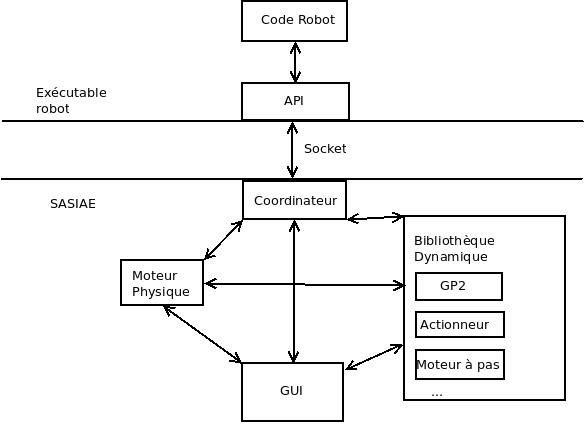
\includegraphics[scale=0.80]{architecture.png}
%\caption{shéma de l'architecture globale de SASIAE}
%\label{figurearchitecture}
%\end{figure}
%\vspace{5 mm}

%\newpage

La figure \ref{messagearchitecture} présente de façon un peu plus détaillée les messages envoyés entre les différents composants du simulateur.
L'objet "Module" est un module générique qui peut être un capteur et un actionneur, il y aura dans l'application plusieurs modules, mais le schéma 
n'en comporte qu'un pour des soucis de lisibilité.

%% Clément : C'est quoi ce "ClientCoordination" côté exécutable robot qui reçoit les valeurs des capteurs ? C'est Aversive++ qui est aussi censé gérer et fournir une abstraction des capteurs !!!

\begin{figure}
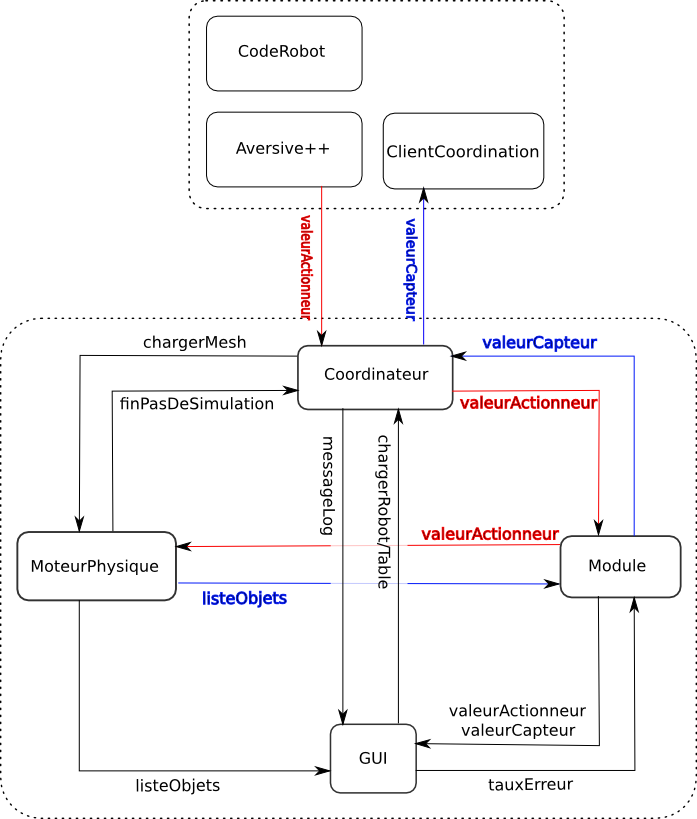
\includegraphics[scale=0.70]{architecturemsg.png}
\caption{messages entre les composants de l'architecture}
\label{messagearchitecture}
\end{figure}
\vspace{5 mm}
